\documentclass{standalone}

\usepackage{tikz}
\usepackage{pgfplots}
\usepackage{verbatim}

\pgfplotsset{ every non boxed x axis/.append style={x axis line style=-},
     every non boxed y axis/.append style={y axis line style=-}}     
\pgfplotsset{compat = 1.9}

\begin{document}
\scriptsize

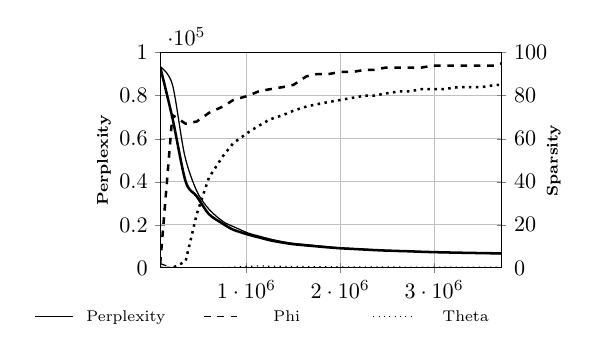
\begin{tikzpicture}[remember picture, baseline=0pt, scale = 0.8]
    \begin{axis}[
        ylabel shift = -3 pt,
        width=7cm,
        height=5cm,
        axis lines=left,
        ymajorgrids=true,
        xmajorgrids=true,
        ymin = 0, ymax = 100000,
        major grid style={draw=lightgray},
        ylabel={\scriptsize $\mathrm{\bf Perplexity}$},
        scaled x ticks = false,                    
        ]
    \addplot[smooth,line width=0.4mm] plot coordinates {
		(80000, 93308)
		(210000, 69748)
		(350000, 40293)
		(470000, 33250)
		(600000, 24970)
		(750000, 20488)
		(860000, 17735)
		(1020000, 15461)
		(1130000, 14215)
		(1250000, 12848)
		(1390000, 11726)
		(1500000, 11023)
		(1640000, 10443)
		(1750000, 10016)
		(1870000, 9555)
		(2000000, 9128)
		(2130000, 8829)
		(2260000, 8527)
		(2360000, 8300)
		(2480000, 8071)
		(2630000, 7858)
		(2740000, 7713)
		(2860000, 7511)
		(2990000, 7345)
		(3100000, 7227)
		(3260000, 7084)
		(3360000, 6996)
		(3508494, 6889)
		(3658494, 6781)
		(3718494, 6723)
    }; \label{perplexityPlsa}
    
    \addplot[smooth,line width=0.2mm] plot coordinates {
		(80000, 93470)
		(210000, 85201)
		(340000, 52457)
		(470000, 35692)
		(600000, 27265)
		(750000, 21531)
		(860000, 19200)
		(1020000, 16156)
		(1130000, 14820)
		(1250000, 13445)
		(1390000, 12148)
		(1500000, 11393)
		(1640000, 10815)
		(1760000, 10255)
		(1870000, 9812)
		(2010000, 9290)
		(2140000, 8958)
		(2250000, 8663)
		(2350000, 8418)
		(2480000, 8149)
		(2620000, 7908)
		(2730000, 7750)
		(2850000, 7536)
		(2990000, 7303)
		(3100000, 7178)
		(3260000, 7016)
		(3360000, 6926)
		(3518494, 6786)
		(3658494, 6670)
		(3718494, 6623)    
    }; \label{perplexityLda}
    \end{axis}
    
    \begin{axis}[
    	ylabel shift = -7 pt,
        width=7cm,
        height=5cm,
        axis lines=left,
        axis x line*=top,
        xtick=\empty,
        axis y line*=right,
        ymin = 0, ymax = 100,
        ylabel near ticks,             
        ylabel={\scriptsize $\mathrm{\bf Sparsity}$},
        legend columns=3, 
        legend style={
            text width=5.5em,
            text height=1.5ex,
            text depth=.5ex,        
        	draw=none,
            /tikz/column 3/.style={
                column sep=0pt,
            },
            at={(axis description cs:1.14,-0.14)}
        },
        every axis legend/.append style={nodes={right}},
        ]
    \addlegendimage{black}        
    \addlegendimage{dashed, black} 
    \addlegendimage{dotted, black}
    \addlegendimage{/pgfplots/refstyle=perplexityPlsa}\addlegendentry{\scriptsize $\mathrm{\:\; Perplexity}$} 
    \addplot[dashed,line width=0.4mm] plot coordinates {
		(80000, 2)
		(210000, 71)
		(350000, 67)
		(470000, 68)
		(600000, 72)
		(750000, 75)
		(860000, 78)
		(1020000, 80)
		(1130000, 82)
		(1250000, 83)
		(1390000, 84)
		(1500000, 85)
		(1640000, 89)
		(1750000, 90)
		(1870000, 90)
		(2000000, 91)
		(2130000, 91)
		(2260000, 92)
		(2360000, 92)
		(2480000, 93)
		(2630000, 93)
		(2740000, 93)
		(2860000, 93)
		(2990000, 94)
		(3100000, 94)
		(3260000, 94)
		(3360000, 94)
		(3508494, 94)
		(3658494, 94)
		(3718494, 95)
    };           
    \addlegendentry{\scriptsize $\mathrm{\hphantom{A}\hphantom{A}Phi}$}

    \addplot[dashed,line width=0.2mm] plot coordinates {
		(80000, 2)
		(210000, 0)
		(340000, 0)
		(470000, 0)
		(600000, 0)
		(750000, 0)
		(860000, 0)
		(1020000, 0)
		(1130000, 0)
		(1250000, 0)
		(1390000, 0)
		(1500000, 0)
		(1640000, 0)
		(1760000, 0)
		(1870000, 0)
		(2010000, 0)
		(2140000, 0)
		(2250000, 0)
		(2350000, 0)
		(2480000, 0)
		(2620000, 0)
		(2730000, 0)
		(2850000, 0)
		(2990000, 0)
		(3100000, 0)
		(3260000, 0)
		(3360000, 0)
		(3518494, 0)
		(3658494, 0)
		(3718494, 0)
    };
    
    \addplot[dotted,line width=0.4mm] plot coordinates {
		(80000, 0)
		(210000, 0)
		(350000, 3)
		(470000, 25)
		(600000, 42)
		(750000, 52)
		(860000, 58)
		(1020000, 63)
		(1130000, 66)
		(1250000, 69)
		(1390000, 71)
		(1500000, 73)
		(1640000, 75)
		(1750000, 76)
		(1870000, 77)
		(2000000, 78)
		(2130000, 79)
		(2260000, 80)
		(2360000, 80)
		(2480000, 81)
		(2630000, 82)
		(2740000, 82)
		(2860000, 83)
		(2990000, 83)
		(3100000, 83)
		(3260000, 84)
		(3360000, 84)
		(3508494, 84)
		(3658494, 85)
		(3718494, 85)
    };         
    \addlegendentry{\scriptsize $\mathrm{\hphantom{A}\hphantom{A}Theta}$}  
    
    \addplot[dotted,line width=0.2mm] plot coordinates {
		(80000, 0.000000)
		(210000, 0.000000)
		(340000, 0.010000)
		(470000, 0.010000)
		(600000, 0.030000)
		(750000, 0.140000)
		(860000, 0.340000)
		(1020000, 0.700000)
		(1130000, 0.880000)
		(1250000, 0.800000)
		(1390000, 0.720000)
		(1500000, 0.650000)
		(1640000, 0.610000)
		(1760000, 0.560000)
		(1870000, 0.530000)
		(2010000, 0.490000)
		(2140000, 0.460000)
		(2250000, 0.440000)
		(2350000, 0.420000)
		(2480000, 0.400000)
		(2620000, 0.380000)
		(2730000, 0.360000)
		(2850000, 0.350000)
		(2990000, 0.330000)
		(3100000, 0.320000)
		(3260000, 0.300000)
		(3360000, 0.290000)
		(3518494, 0.280000)
		(3658494, 0.270000)
		(3718494, 0.270000)	
    };
    \end{axis}
\end{tikzpicture}
\normalsize

\end{document}